
In questa sezione verrà riportato il bilancio delle ore dei vari componenti del gruppo in base ai ruoli sostenuti. Il bilancio sarà così analizzato:
\begin{itemize}
	\item {\bfseries in positivo}: se il numero delle ore effettuate è minore rispetto a quelle preventivate;
	\item {\bfseries in negativo}: se il numero delle ore effettuate è maggiore rispetto a quelle preventivate;
	\item {\bfseries in pari}: se il numero delle ore effettuate è uguale rispetto a quelle preventivate. \\
\end{itemize}
Nella sezione che interessa il prospetto economico, in cui sono riportate le ore totali per ciascun costo, verranno analizzate nel seguente modo:
\begin{itemize}
	\item {\bfseries in positivo}: la somma finale è minore rispetto a quella preventivata, il proponente ha risparmiato denaro;
	\item {\bfseries in negativo}: la somma finale è maggiore rispetto a quella preventivata, il proponente ha investito più denaro;
	\item {\bfseries in pari}: la somma finale è invariata rispetto a quanto preventivato. \\
\end{itemize}
\subsection {Analisi dei requisiti}
\subsubsection{Prospetto orario}
	\begin{table} [h!]
	\begin{center}
		\rowcolors{2}{gray!25}{gray!6}
		\begin{tabular} {m{3.5cm} c c c c c c c }
			\rowcolor{lightgray}
			\textbf{Nome} & \textbf{Re} & \textbf{Am} & \textbf{An} & \textbf{Pg} &\textbf{Pr} & \textbf{Ve} & \textbf{Totale} \\ 
			Matteo Alba & 0 & 8(-5) &8(+4) & 0 & 0 & 10(+1) & 26  \\ 
			Giacomo Bulbarelli & 7(+4) & 6(-1) & 8(-2) & 0 & 0 & 5(-1) & 26 \\ 
			Alessandro Chimetto & 7 & 0(-4) & 11(+4) & 0 & 0 & 8 & 26 \\
			Alessandro Dindinelli & 0 & 4(-1) & 12(+1) & 0 & 0 & 10 & 26 \\
			Lucia Fenu & 0(-3) & 6(-4) & 10(+6) & 0 & 0 & 10(+1) & 26 \\
			Paolo Scanferlato & 5(+1) & 7(-4) & 6(+2) & 0 & 0 & 8(+1) & 26 \\
			Valton Tahiraj & 6(+3) & 5(-2) &7(+1) & 0 & 0 & 8(-2) & 26 \\
			\textbf{Ore Totali Ruolo} & \textbf{25(+5)} & \textbf{36(-21)} & \textbf{62(+16)} & \textbf{0} & \textbf{0} & \textbf{59} & \textbf{182}\\
		
		\end{tabular}
		\caption{Consuntivo - Analisi dei requisiti - ore per persona/ruolo}
	\end{center}
\end{table}

	\begin{figure} [h!]
	\centering
	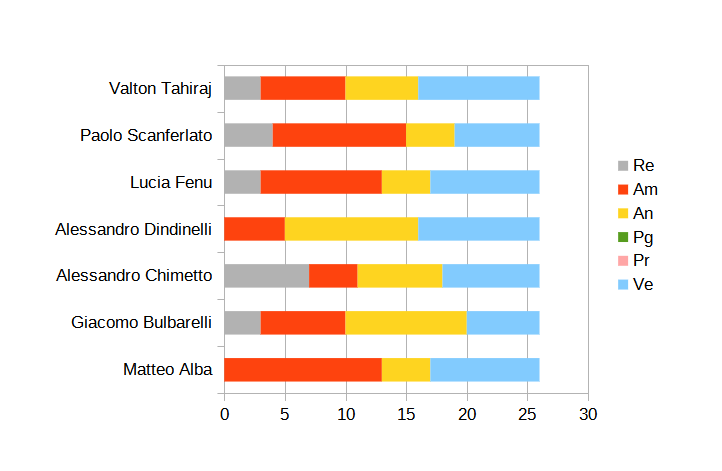
\includegraphics[width=0.7\textwidth]{res/img/grafici/consuntivo-barre_ ore analisi requisiti.png}
	\caption{Consuntivo - Analisi dei requisiti - ore per persona/ruolo} 
\end{figure}


\newpage
\subsubsection{Prospetto economico}


\begin{table} [h!]
	\begin{center}
		\rowcolors{2}{gray!25}{gray!6}
		\begin{tabular} { m{3 cm} c c c  }
			\rowcolor{lightgray}
			\textbf{Ruolo} & \textbf{Ore} & \textbf{Costo in \euro} \\
			Responsabile & 25(+5) & 750,00 (+150,00) \\
			Amministratore & 36(-21) & 720,00 (-420,00)  \\
			Analista & 62(+16) & 1550,00 (+400,00) \\
			Progettista & 0 & 0 \\
			Programmatore & 0 & 0  \\
			Verificatore & 59 & 885,00  \\
			\textbf{Totale} & \textbf{182}  & \textbf{3905,00 (+130,00)} \\
			
		\end{tabular}
		\caption{Consuntivo - Analisi dei requisiti - costo per ruolo}
	\end{center}
\end{table}

\begin{figure} [h!]
	\centering
	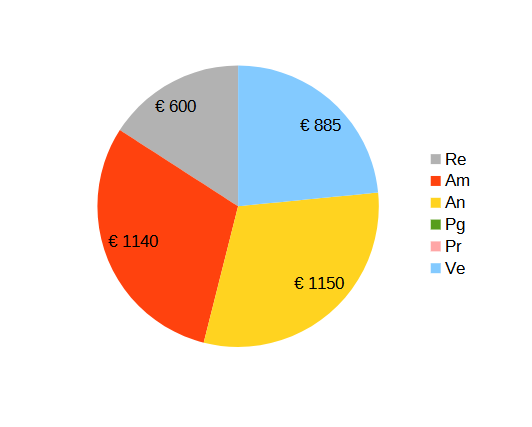
\includegraphics[width=0.6\textwidth]{res/img/grafici/consuntivo- torta_ costo_per_ora- analisi dei requisiti.png}
	\caption{Consuntivo - Analisi dei requisiti - costo per ruolo} 
\end{figure}

\newpage 

\subsubsection{Conclusioni}
Il gruppo nel complesso, ha lavorato secondo le ore preventivate seppur con alcune modifiche nella rotazione dei ruoli.
Nello specifico:
\begin{itemize}
	\item {\bfseries responsabile}: le ore previste, nel complesso, sono state rispettate. Per parallelizzare meglio il lavoro, è stato incluso un membro all'interno del ruolo (rispetto al preventivo), alleggerendo anche il carico ad altri membri;
	\item {\bfseries amministratore}: il lavoro previsto per la stesura dei documenti ha richiesto più ore rispetto a quelle preventivate, distribuite su tutti i membri;
	\item {\bfseries analista}: la stesura dell'\dext{Analisi dei requisiti} ha richiesto meno tempo rispetto a quanto preventivato e dunque, le ore mancanti, sono state distribuite nei restanti ruoli che ne necessitavano di più;
	\item {\bfseries verificatore}: grazie all'attenzione riposta nella gestione dei documenti, è stato svolto il ruolo di verificatore nelle ore previste.\\
		
	A causa della variazione oraria di alcuni ruoli, il totale prevede una spesa inferiore di \euro 130,00 rispetto a quanto preventivato.
	Tuttavia, la fase di analisi dei requisiti, non è rendicontata.
	
\end{itemize}



	

	
\newpage	
	
\subsection{ Analisi di dettaglio}


\subsubsection{Prospetto orario}
	\begin{table} [h!]
	\rowcolors{2}{gray!25}{gray!6}
	\begin{center}
		\begin{tabular} {m{3.5cm} c c c c c c c  }
			\rowcolor{lightgray}
			\textbf{Nome} & \textbf{Re} & \textbf{Am} & \textbf{An} & \textbf{Pg} & \textbf{Pr} & \textbf{Ve} & \textbf{Totale} \\
			Matteo Alba               & 2(+2) & 0(-2) & 0      & 0  & 0  & 4      & 6 \\
			Giacomo Bulbarelli        & 0     & 2     & 4      & 0  & 0  & 0      & 6 \\
			Alessandro Chimetto       & 0(-1) & 5(+2) & 1(-1)  & 0  & 0  & 0      & 6 \\
			Alessandro Dindinelli     & 3     & 0(-2) & 1(+1)  & 0  & 0  & 2(+1)  & 6 \\
			Lucia Fenu                & 1     & 0(-2) & 3(+2)  & 0  & 0  & 2      & 6 \\
			Paolo Scanferlato         & 0     & 0     & 2      & 0  & 0  & 4      & 6 \\
			Valton Tahiraj            & 0     & 0     & 3(+1)  & 0  & 0  & 3(-1)  & 6\\
			\textbf{Ore totali Ruolo} & \textbf{6(+1)} & \textbf{7(-4)} & \textbf{14(+3)} & \textbf{0}  & \textbf{0}  & \textbf{15}     & \textbf{42}
		\end{tabular}
		\caption{Consuntivo - Analisi di dettaglio - ore per persona/ruolo}
	\end{center}
\end{table}

	\begin{figure} [h!]
	\centering
	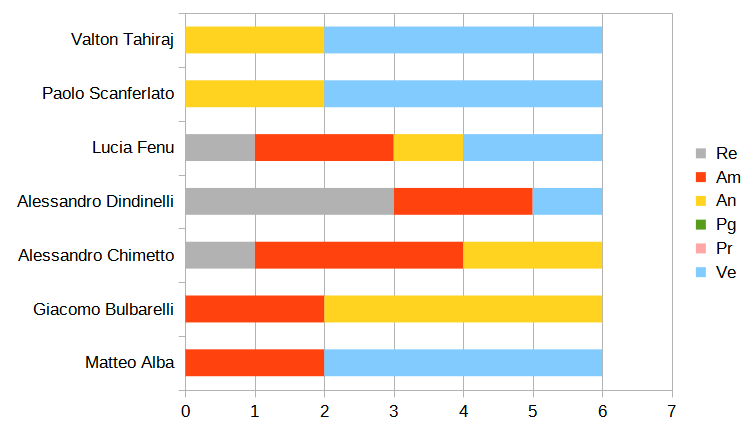
\includegraphics[width=0.7\textwidth]{res/img/grafici/consuntivo-barre- ore analisi dettaglio.png}
	\caption{Consuntivo - Analisi di dettaglio -  ore per persona/ruolo} 
\end{figure}

\newpage
\subsubsection{Prospetto economico}


\begin{table} [h!]
	\begin{center}
		\rowcolors{2}{gray!25}{gray!6}
		\begin{tabular} { m{3 cm} c c c  }
			\rowcolor{lightgray}
			\textbf{Ruolo}  & \textbf{Ore} & \textbf{Costo in \euro} \\
			Responsabile    & 6(+1)      & 180,00 (+30,00) \\
			Amministratore  & 7(-4)      & 140,00 (-80,00)  \\
			Analista        & 14(+3)     & 350,00 (+75,00) \\
			Progettista     & 0          & 0 \\
			Programmatore   & 0          & 0  \\
			Verificatore    & 15         & 225,00  \\
			\textbf{Totale} & \textbf{42}         & \textbf{895,00 (+25,00)} \\
			
		\end{tabular}
		\caption{Consuntivo - Analisi di dettaglio - costo per ruolo}
	\end{center}
\end{table}
	\begin{figure} [h!]
	\centering
	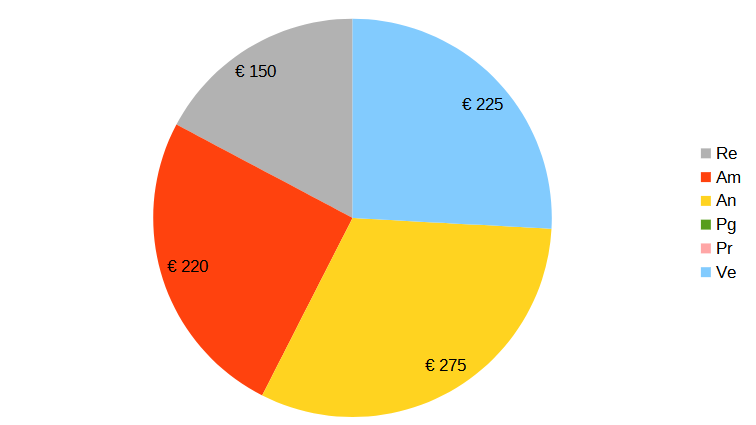
\includegraphics[width=0.7\textwidth]{res/img/grafici/consuntivo-torta-analisi di dettaglio.png}
	\caption{Consuntivo - Analisi di dettaglio - costo per ruolo} 
\end{figure}

\subsubsection{Conclusioni }
In conclusione, si osserva un risparmio orario nei ruoli di Responsabile e Analista compensato dall'investimento orario parallelo nel ruolo di Amministratore.\\
Dal punto di vista economico si osserva un leggero risparmio dei costi previsti. \\
In generale, il preventivo era corretto ma non erano previsti oneri amministrativi come quelli incontrati.


\newpage

\subsection{Codifica \glock{Technlogy Baseline}}

\subsubsection{Prospetto orario}
\begin{table} [h!]
	\rowcolors{2}{gray!25}{gray!6}
	\begin{center}
		\begin{tabular} { m{3.5cm} c c c c c c c }
			\rowcolor{lightgray}
			\textbf{Nome} & \textbf{Re} & \textbf{Am} & \textbf{An} & \textbf{Pg} & \textbf{Pr} & \textbf{Ve} & \textbf{Totale} \\
			Matteo Alba               & 8(+3)      & 0(-3)    & 4      & 3  & 5  & 6      & 27 \\
			Giacomo Bulbarelli        & 3     & 0     & 5(+2)  & 7  & 5(-4)  & 7(+2)      & 27 \\
			Alessandro Chimetto       & 0     & 2    & 4(+2)       & 6(-1)  & 6(-1)  & 9     & 27 \\
			Alessandro Dindinelli     & 2     & 4    & 0       & 7  & 7  & 7  & 27 \\
			Lucia Fenu                & 0(-2)  & 2(-2)  & 3      & 7(+2)   & 7(+2)   & 9      & 27 \\
			Paolo Scanferlato         & 2      & 3      & 3      & 6       & 4       & 9      & 27 \\
			Valton Tahiraj            & 0      & 3      & 4(+2)  & 3(-2)   & 6(-2)   & 11(+2) & 27\\
			\textbf{Ore totali Ruolo} & \textbf{15(+1)} & \textbf{14(-5)} & \textbf{23(+6)} & \textbf{39(-1)}  & \textbf{40(-5)}  & \textbf{58(+4)} & \textbf{189}\\
		\end{tabular}
		\caption{Consuntivo - Codifica \glock{Technlogy Baseline} - ore per persona/ruolo}
	\end{center}
\end{table}
	\begin{figure} [h!]
	\centering
	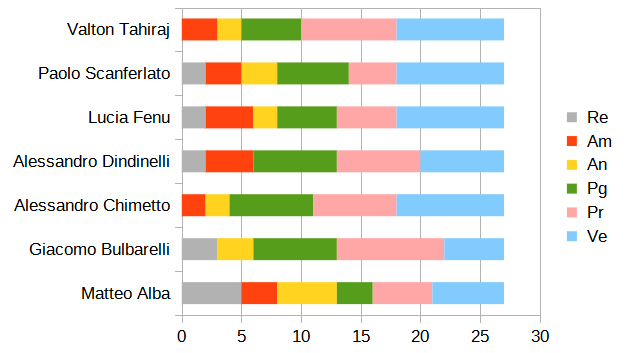
\includegraphics[width=0.7\textwidth]{res/img/grafici/consuntivo-barre-tb.png}
	\caption{Consuntivo - Codifica \glock{Technlogy Baseline} -  ore per persona/ruolo} 
\end{figure}
\newpage
\subsubsection{Prospetto economico}


\begin{table} [h!]
	\begin{center}
		\rowcolors{2}{gray!25}{gray!6}
		\begin{tabular} { m{3 cm} c c c  }
			\rowcolor{lightgray}
			\textbf{Ruolo}  & \textbf{Ore} & \textbf{Costo in \euro} \\
			Responsabile    & 15(+1)      & 450,00 (+30,00) \\
			Amministratore  & 14(-5)      & 280,00 (-100,00)  \\
			Analista        & 23(+6)     & 575,00 (+150,00) \\
			Progettista     & 39(-1)          & 858,00 (-22,00) \\
			Programmatore   & 40(-5)        & 600,00 (-75,00) \\
			Verificatore    & 58(+4)        & 870,00 (+60,00) \\
			\textbf{Totale} & \textbf{189}         & \textbf{3633,00 (+43,00)} \\
			
		\end{tabular}
		\caption{Consuntivo - Codifica \glock{Technlogy Baseline} - costo per ruolo}
	\end{center}
\end{table}
\begin{figure} [h!]
	\centering
	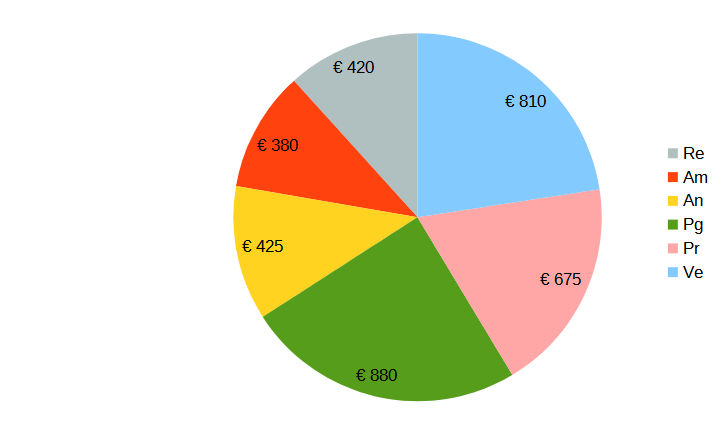
\includegraphics[width=0.7\textwidth]{res/img/grafici/consuntivo-torta-tb.png}
	\caption{Consuntivo - Codifica \glock{Technlogy Baseline} - costo per ruolo} 
\end{figure}
\subsubsection{Conclusioni}
L'impegno orario preventivato è corretto rispetto al totale monte ore.\\ Decisamente meno il prospetto orario di dettaglio sui singoli ruoli: il lavoro svolto si è incentrato molto di più sulla codifica e sulla progettazione, mentre (complice un workflow funzionale e una necessità meno stringente di verificare il codice prodotto), i ruoli di Analista e Verificatore sono risultati meno importanti del previsto.\\
Il risparmio anche in questo caso è significativo nel sottolineare come il preventivo orario sia corretto rispetto al monte ore finale ma da rivedere rispetto all'impegno che il singolo ruolo ha nella fase specifica di cui si fa preventivo. \\ 

\newpage
\subsection{Progettazione Architetturale}
\subsubsection{Prospetto orario}

\begin{table} [h!]
	\rowcolors{2}{gray!25}{gray!6}
	\begin{center}
		\begin{tabular} { m{3.5cm} c c c c c c c }
			\rowcolor{lightgray}
			\textbf{Nome} & \textbf{Re} & \textbf{Am} & \textbf{An} & \textbf{Pg} & \textbf{Pr} & \textbf{Ve} & \textbf{Totale} \\
			Matteo Alba & 0 & 2 & 2 & 13(+3) & 0 & 3 & 20(+3) \\
			Giacomo Bulbarelli & 0 & 0 & 0 & 17(-10) & 0 & 3(-1) & 20(-11) \\
			Alessandro Chimetto & 0 & 0 & 2 & 16(-13) & 0 & 2(+2) & 20(-11) \\
			Alessandro Dindinelli & 0 & 2 & 2 & 16(-11) & 0 & 0 & 20(-11) \\
			Lucia Fenu & 2 & 0 & 0 & 16(-11) & 0 & 2 & 20(-11) \\
			Paolo Scanferlato & 2 & 0 & 0 & 16(-11) & 0 & 2 & 20(-11) \\
			Valton Tahiraj & 0 & 0 & 0 & 17(-9) & 0 & 3(-2) & 20(-11)\\
			\textbf{Ore totali Ruolo} & \textbf{4} & \textbf{4} & \textbf{6} & \textbf{111(-62)} & \textbf{0}& \textbf{15(-1)} & \textbf{140(-63)}
		\end{tabular}
		\caption{Preventivo - Progettazione architetturale - ore per persona/ruolo}
	\end{center}
\end{table}

\begin{figure} [h!]
	\centering
	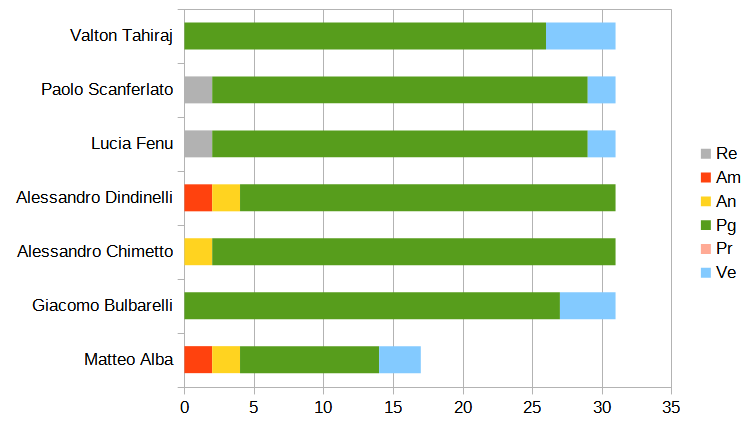
\includegraphics[width=0.8\textwidth]{res/img/grafici/consuntivo-barre- ore progettazione.png}
	\caption{Preventivo - Progettazione architetturale -ore per persona/ruolo} 
\end{figure}

\newpage

\subsubsection{Prospetto economico}

\begin{table} [h!] % QUESTA RICHIEDE \usepackage{eurosym} IN config.tex
	\rowcolors{2}{gray!25}{gray!6}
	\begin{center}
		\begin{tabular} { m{3cm} >{\centering}m{1.5cm} c }
			\rowcolor{lightgray}
			\textbf{Ruolo} & \textbf{Ore} & \textbf{Costo in \euro} \\
			Responsabile & 4 & 120,00 \\
			Amministratore & 4 & 80,00 \\
			Analista & 6 & 150,00 \\
			Progettista & 111(-62) & 2442,00(-1364,00)\\
			Programmatore & 0 & 0,00 \\
			Verificatore & 15(-1) & 225,00(-15,00) \\
			\textbf{Totale} & \textbf{140(-63} & \textbf{3017,00(-1379,00)} \\
		\end{tabular}
		\caption{Preventivo - Progettazione architetturale - costo per ruolo}
	\end{center}
\end{table}

\begin{figure} [h!]
	\centering
	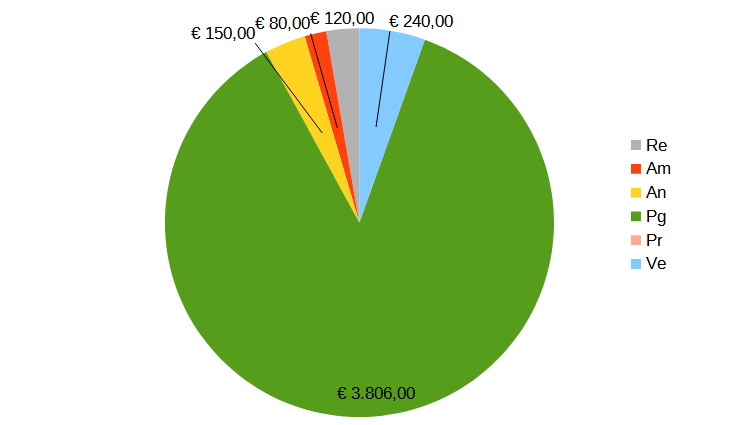
\includegraphics[width=0.8\textwidth]{res/img/grafici/consuntivo-torta-progettazione.png}
	\caption{Preventivo - Progettazione architetturale - costo per ruolo} 
\end{figure}
\subsubsection{Conclusioni}
Lo svolgimento della Progettazione architetturale non è andata quanto previsto a causa di una errata pianificazione e sottovalutazione del lavoro da svolgere. Infatti il consuntivo rispecchia questa discrepanza.
Il gruppo nel complesso ha lavorato bene.


\newpage

\subsection{Incremento I}
\subsubsection{Prospetto orario}

\begin{table} [h!]
	\rowcolors{2}{gray!25}{gray!6}
	\begin{center}
		\begin{tabular} { m{3.5cm} c c c c c c c }
			\rowcolor{lightgray}
			\textbf{Nome} & \textbf{Re} & \textbf{Am} & \textbf{An} & \textbf{Pg} & \textbf{Pr} & \textbf{Ve} & \textbf{Totale} \\
			Matteo Alba & 1 & 0 & 0 & 0 & 3 & 3 & 7 \\
			Giacomo Bulbarelli & 1 & 0 & 0 & 0 & 4(-6) & 2(-1) & 7(-7) \\
			Alessandro Chimetto & 0 & 0 & 0 & 1 & 4(-6) & 2(-1) & 7(-7) \\
			Alessandro Dindinelli & 0 & 0 & 1 & 0 & 4(-6) & 2(-1) & 7 (-7)\\
			Lucia Fenu & 0 & 2 & 0 & 1(-2) & 4(-4) & 0 (-1)& 7 (-7)\\
			Paolo Scanferlato & 0 & 0 & 0 & 1 & 2(-6) & 4(-1) & 7(-7) \\
			Valton Tahiraj & 0 & 0 & 0 & 1(-1) & 4(-4) & 2(-2) & 7(-7) \\
			\textbf{Ore totali Ruolo} & \textbf{2} & \textbf{2} & \textbf{1} & \textbf{4(-3)} & \textbf{25(-32)}& \textbf{15(-7)} & \textbf{49(-42)}
		\end{tabular}
		\caption{Preventivo - Incremento I - ore per persona/ruolo}
	\end{center}
\end{table}
\begin{figure} [h!]
	\centering
	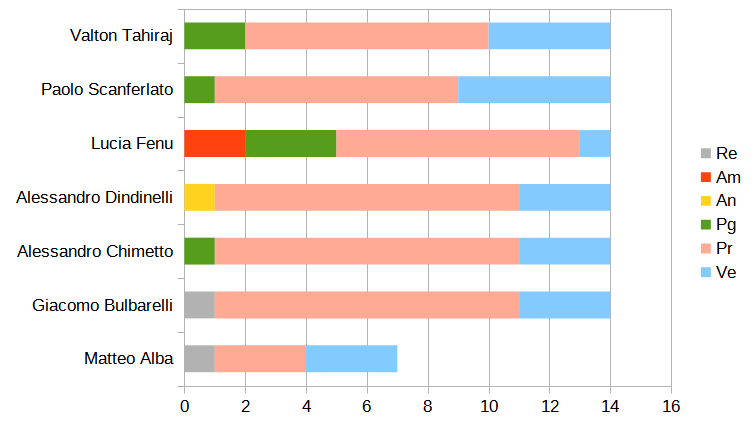
\includegraphics[width=0.8\textwidth]{res/img/grafici/consuntivo-barre- incremento1.png}
	\caption{Preventivo - Incremento I - ore per persona/ruolo} 
\end{figure}

\newpage

\subsubsection{Prospetto economico}
\begin{table} [h!] % QUESTA RICHIEDE \usepackage{eurosym} IN config.tex
	\rowcolors{2}{gray!25}{gray!6}
	\begin{center}
		\begin{tabular} { m{3cm} >{\centering}m{1.5cm} c }
			\rowcolor{lightgray}
			\textbf{Ruolo} & \textbf{Ore} & \textbf{Costo in \euro} \\
			Responsabile & 2 & 60,00 \\
			Amministratore & 2 & 40,00 \\
			Analista & 1 & 25,00 \\
			Progettista & 4(-3) & 88,00(-66,00) \\
			Programmatore & 25(-32) & 375,00(-480,00) \\
			Verificatore & 15(-7) & 225,00(-105,00)\\
			\textbf{Totale} & \textbf{49(-42)} & \textbf{813,00(-651,00)} \\
		\end{tabular}
		\caption{Preventivo - Incremento I - costo per ruolo}
	\end{center}
\end{table}

\begin{figure} [h!]
	\centering
	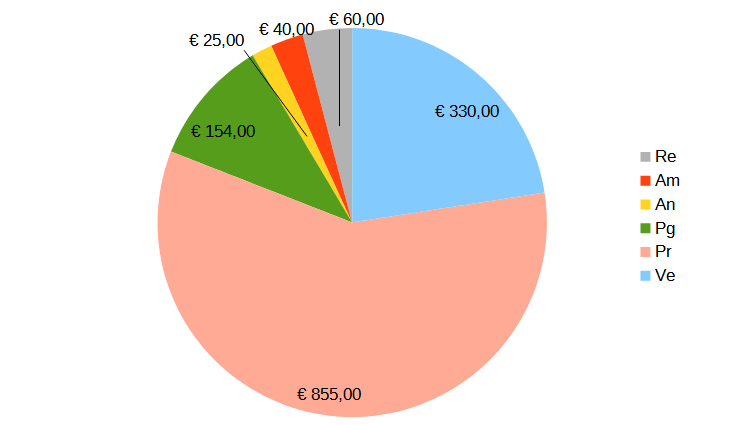
\includegraphics[width=0.8\textwidth]{res/img/grafici/consuntivo-torta-incremento1.png}
	\caption{Preventivo - Incremento I - costo per ruolo} 
\end{figure}


\newpage
\subsection{Incremento II}
\subsubsection{Prospetto orario}

\begin{table} [h!]
	\rowcolors{2}{gray!25}{gray!6}
	\begin{center}
		\begin{tabular} { m{3.5cm} c c c c c c c }
			\rowcolor{lightgray}
			\textbf{Nome} & \textbf{Re} & \textbf{Am} & \textbf{An} & \textbf{Pg} & \textbf{Pr} & \textbf{Ve} & \textbf{Totale} \\
			Matteo Alba & 0 & 2 & 1 & 0 & 3(+1) & 1 & 7(+1) \\
			Giacomo Bulbarelli & 0 & 0 & 0 & 0 & 5(-2) & 1(-1) & 6(-3) \\
			Alessandro Chimetto & 1 & 0 & 0 & 0 & 4(-3) & 2 & 7(-3) \\
			Alessandro Dindinelli & 0 & 0 & 0 & 1 & 4(-3) & 2 & 7(-3) \\
			Lucia Fenu & 0 & 0 & 0 & 0 & 4(-3) & 3 & 7(-3) \\
			Paolo Scanferlato & 0 & 1 & 0 & 0 & 5(-2) & 1(-1) & 7(-3) \\
			Valton Tahiraj & 0 & 0 & 0 & 1 & 2(-3) & 4 & 7 (-3)\\
			\textbf{Ore totali Ruolo} & \textbf{1} & \textbf{3} & \textbf{1} & \textbf{2} & \textbf{27(-15)}& \textbf{14(-2)} & \textbf{48(-18)}
		\end{tabular}
		\caption{Preventivo - Incremento II - ore per persona/ruolo}
	\end{center}
\end{table}
\begin{figure} [h!]
	\centering
	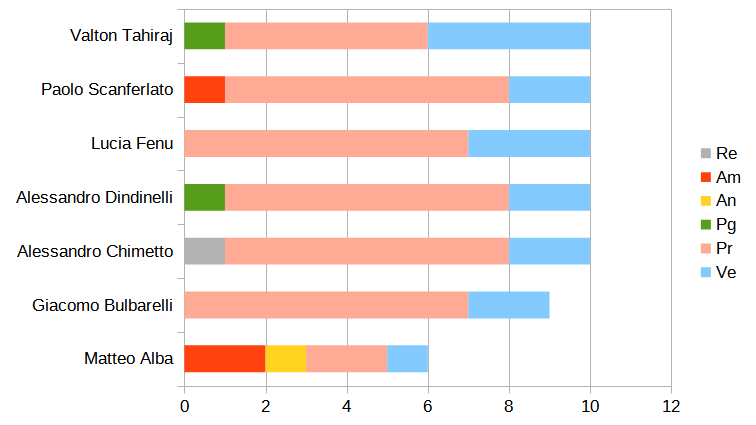
\includegraphics[width=0.8\textwidth]{res/img/grafici/consuntivo-barre- incremento2.png}
	\caption{Preventivo - Incremento II - ore per persona/ruolo} 
\end{figure}

\newpage

\subsubsection{Prospetto economico}
\begin{table} [h!] % QUESTA RICHIEDE \usepackage{eurosym} IN config.tex
	\rowcolors{2}{gray!25}{gray!6}
	\begin{center}
		\begin{tabular} { m{3cm} >{\centering}m{1.5cm} c }
			\rowcolor{lightgray}
			\textbf{Ruolo} & \textbf{Ore} & \textbf{Costo in \euro} \\
			Responsabile &1 & 30,00 \\
			Amministratore & 3 & 60,00 \\
			Analista &1 & 25,00 \\
			Progettista & 2 & 44,00 \\
			Programmatore & 27(-15) & 405,00(-225,00)\\
			Verificatore & 14(-2) & 210,00(-30,00) \\
			\textbf{Totale} & \textbf{48(-17)} & \textbf{774,00(-255,00)} \\
		\end{tabular}
		\caption{Preventivo - Incremento II - costo per ruolo}
	\end{center}
\end{table}

\begin{figure} [h!]
	\centering
	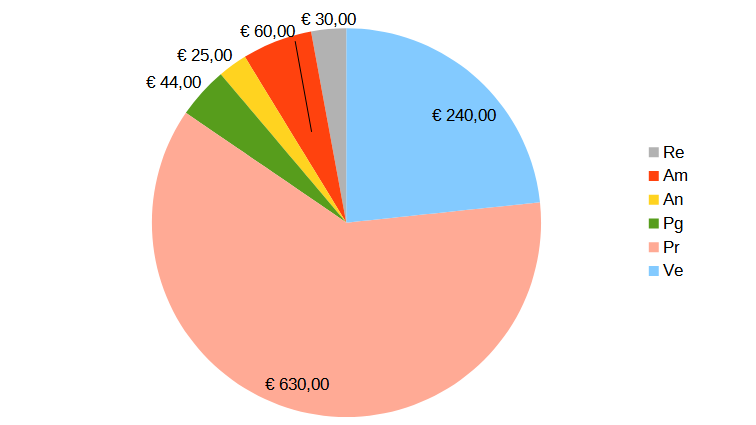
\includegraphics[width=0.8\textwidth]{res/img/grafici/consuntivo-torta-incremento2.png}
	\caption{Preventivo - Incremento II - costo per ruolo} 
\end{figure}
\newpage
\subsection{Incremento III}
\subsubsection{Prospetto orario}

\begin{table} [h!]
	\rowcolors{2}{gray!25}{gray!6}
	\begin{center}
		\begin{tabular} { m{3.5cm} c c c c c c c }
			\rowcolor{lightgray}
			\textbf{Nome} & \textbf{Re} & \textbf{Am} & \textbf{An} & \textbf{Pg} & \textbf{Pr} & \textbf{Ve} & \textbf{Totale} \\
			Matteo Alba & 0 & 1 & 1 & 0 & 4(+2) & 2 & 8(+2) \\
			Giacomo Bulbarelli & 0 & 1 & 0 & 1 & 4(-3) & 2 & 8(-3) \\
			Alessandro Chimetto & 0 & 0 & 0 & 0 & 4(-3) & 3 & 7(-3)\\
			Alessandro Dindinelli & 0 & 0 & 0 & 0 & 4(-3) & 3 & 7(-3) \\
			Lucia Fenu & 1 & 0 & 0 & 0 & 3(-3) & 3 & 7(-3) \\
			Paolo Scanferlato & 0 & 0 & 0 & 0 & 4(-3) & 3 & 7(-3) \\
			Valton Tahiraj & 0 & 0 & 0 & 1(-1) & 5(-1) & 1(-1) & 7(-3) \\
			\textbf{Ore totali Ruolo} & \textbf{1} & \textbf{2} & \textbf{1} & \textbf{2(-1)} & \textbf{28(-14)}& \textbf{17(-1)} & \textbf{51(-16)}
		\end{tabular}
		\caption{Preventivo - Incremento III - ore per persona/ruolo}
	\end{center}
\end{table}
\begin{figure} [h!]
	\centering
	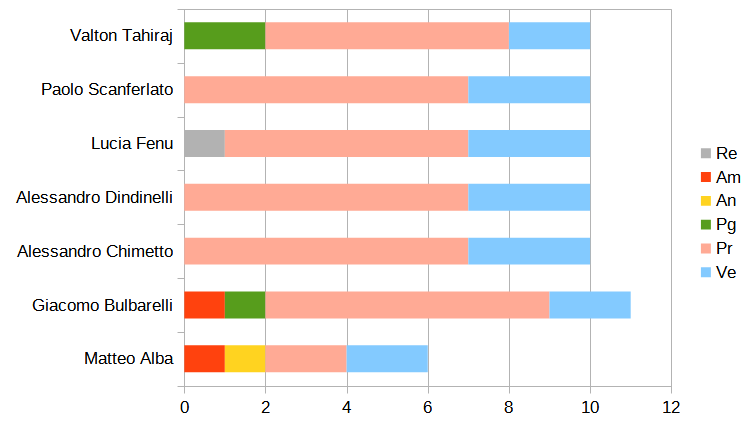
\includegraphics[width=0.8\textwidth]{res/img/grafici/consuntivo-barre- incremento3.png}
	\caption{Preventivo - Incremento III - ore per persona/ruolo} 
\end{figure}

\newpage

\subsubsection{Prospetto economico}
\begin{table} [h!] % QUESTA RICHIEDE \usepackage{eurosym} IN config.tex
	\rowcolors{2}{gray!25}{gray!6}
	\begin{center}
		\begin{tabular} { m{3cm} >{\centering}m{1.5cm} c }
			\rowcolor{lightgray}
			\textbf{Ruolo} & \textbf{Ore} & \textbf{Costo in \euro} \\
			Responsabile & 1 & 30,00 \\
			Amministratore & 2 & 40,00 \\
			Analista & 1 & 25,00 \\
			Progettista & 2(-1) & 44,00(-22,00) \\
			Programmatore & 28(-14) & 420,00(-210,00) \\
			Verificatore & 17(-1)& 255,00(-15,00) \\
			\textbf{Totale} & \textbf{51(-16)} & \textbf{814,00(-247,00)} \\
		\end{tabular}
		\caption{Preventivo - Incremento III - costo per ruolo}
	\end{center}
\end{table}

\begin{figure} [h!]
	\centering
	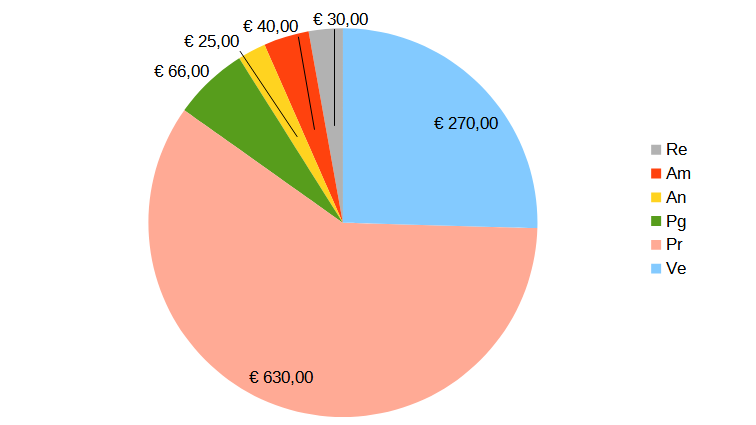
\includegraphics[width=0.8\textwidth]{res/img/grafici/consuntivo-torta-incremento3.png}
	\caption{Preventivo - Incremento III - costo per ruolo} 
\end{figure}
\newpage
\subsection{Incremento IV}
\subsubsection{Prospetto orario}

\begin{table} [h!]
	\rowcolors{2}{gray!25}{gray!6}
	\begin{center}
		\begin{tabular} { m{3.5cm} c c c c c c c }
			\rowcolor{lightgray}
			\textbf{Nome} & \textbf{Re} & \textbf{Am} & \textbf{An} & \textbf{Pg} & \textbf{Pr} & \textbf{Ve} & \textbf{Totale} \\
			Matteo Alba & 0 & 2 & 0 & 0 & 3 & 1 & 6 \\
			Giacomo Bulbarelli & 1 & 0 & 1 & 1 & 1(-2) & 3(-2)& 7(-4) \\
			Alessandro Chimetto & 0 & 0 & 0 & 0 & 3(-4) & 4 & 7(-4) \\
			Alessandro Dindinelli & 0 & 0 & 0 & 0 & 5(-2) & 2(-2) & 7(-4)\\
			Lucia Fenu & 0 & 0 & 0 & 1 & 4(-2) & 2(-2) & 7(-4) \\
			Paolo Scanferlato & 0 & 1 & 0 & 0 & 4(-2) & 2(-2)& 7(-4) \\
			Valton Tahiraj & 0 & 0 & 0 & 0 & 5(-2) & 2(-2)& 7(-4) \\
			\textbf{Ore totali Ruolo} & \textbf{1} & \textbf{3} & \textbf{1} & \textbf{2} & \textbf{25(-13)}& \textbf{16(-12)} & \textbf{48(-25)}
		\end{tabular}
		\caption{Preventivo - Incremento IV - ore per persona/ruolo}
	\end{center}
\end{table}
\begin{figure} [h!]
	\centering
	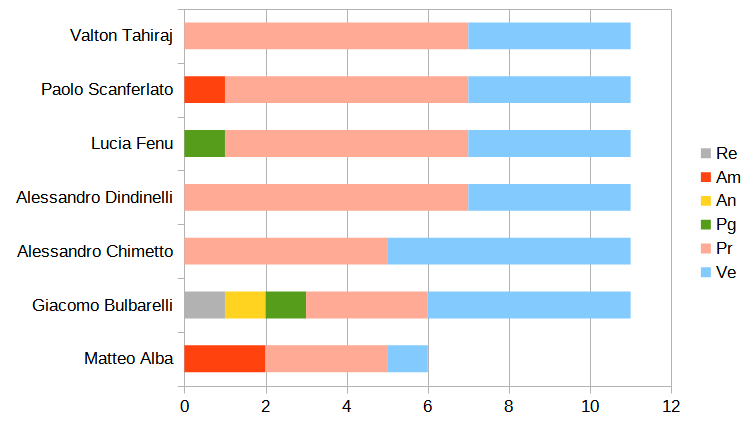
\includegraphics[width=0.8\textwidth]{res/img/grafici/consuntivo-barre- incremento4.png}
	\caption{Preventivo - Incremento IV - ore per persona/ruolo} 
\end{figure}

\newpage
\subsubsection{Prospetto economico}

\begin{table} [h!] % QUESTA RICHIEDE \usepackage{eurosym} IN config.tex
	\rowcolors{2}{gray!25}{gray!6}
	\begin{center}
		\begin{tabular} { m{3cm} >{\centering}m{1.5cm} c }
			\rowcolor{lightgray}
			\textbf{Ruolo} & \textbf{Ore} & \textbf{Costo in \euro} \\
			Responsabile & 1 & 30,00 \\
			Amministratore & 3 & 60,00 \\
			Analista & 1 & 25,00 \\
			Progettista & 2 & 44,00 \\
			Programmatore & 25(-13) & 375,00(-195,00) \\
			Verificatore & 16(-12) & 240,00(-180,00) \\
			\textbf{Totale} & \textbf{48(-25)} & \textbf{774,00(-375,00)} \\
		\end{tabular}
		\caption{Preventivo - Incremento IV - costo per ruolo}
	\end{center}
\end{table}

\begin{figure} [h!]
	\centering
	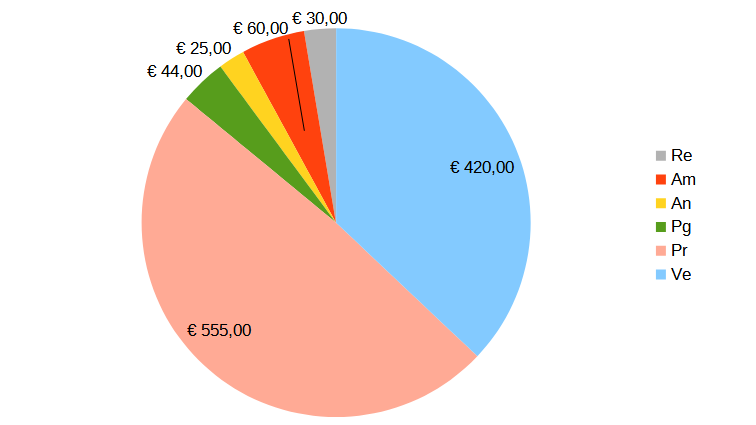
\includegraphics[width=0.8\textwidth]{res/img/grafici/consuntivo-torta-incremento4.png}
	\caption{Preventivo - Incremento IV - costo per ruolo} 
\end{figure}
\newpage
\subsection{Incremento V}
\subsubsection{Prospetto orario}

\begin{table} [h!]
	\rowcolors{2}{gray!25}{gray!6}
	\begin{center}
		\begin{tabular} { m{3.5cm} c c c c c c c }
			\rowcolor{lightgray}
			\textbf{Nome} & \textbf{Re} & \textbf{Am} & \textbf{An} & \textbf{Pg} & \textbf{Pr} & \textbf{Ve} & \textbf{Totale} \\
			Matteo Alba & 0 & 1 & 0 & 0 & 0 & 2 & 3 \\
			Giacomo Bulbarelli & 0 & 3 & 0 & 0 & 0 & 0(-1) & 3(-1) \\
			Alessandro Chimetto & 1 & 2(-1) & 0 & 0 & 0 & 0 & 3(-1)\\
			Alessandro Dindinelli & 0 & 2(-1) & 0 & 0 & 0 & 1 & 3(-1) \\
			Lucia Fenu & 1 & 2(-1) & 0 & 0 & 0 & 0 & 3(-1) \\
			Paolo Scanferlato & 0 & 3(-1) & 0 & 0 & 0 & 0 & 3(-1) \\
			Valton Tahiraj & 0 & 2(-1) & 0 & 0 & 0 & 1 & 3(-1)\\
			\textbf{Ore totali Ruolo} & \textbf{2} & \textbf{15(-5)} & \textbf{0} & \textbf{0} & \textbf{0}& \textbf{4(-1)} & \textbf{21(-6)}
		\end{tabular}
		\caption{Preventivo - Incremento V - ore per persona/ruolo}
	\end{center}
\end{table}
\begin{figure} [h!]
	\centering
	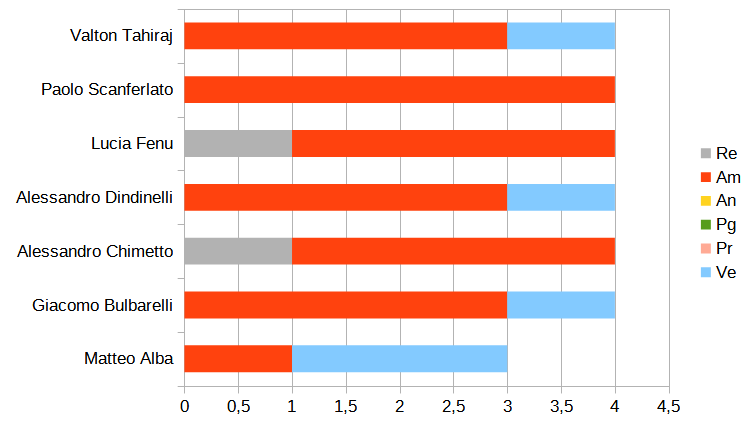
\includegraphics[width=0.8\textwidth]{res/img/grafici/consuntivo-barre- incremento5.png}
	\caption{Preventivo - Incremento V - ore per persona/ruolo} 
\end{figure}

\newpage
\subsubsection{Prospetto economico}
\begin{table} [h!] % QUESTA RICHIEDE \usepackage{eurosym} IN config.tex
	\rowcolors{2}{gray!25}{gray!6}
	\begin{center}
		\begin{tabular} { m{3cm} >{\centering}m{1.5cm} c }
			\rowcolor{lightgray}
			\textbf{Ruolo} & \textbf{Ore} & \textbf{Costo in \euro} \\
			Responsabile & 2 & 60,00 \\
			Amministratore & 15(-5) & 300,00(-100,00) \\
			Analista & 0 & 0,00 \\
			Progettista & 0 & 0,00 \\
			Programmatore & 0 & 0,00 \\
			Verificatore & 4(-1) & 60,00(-15,00) \\
			\textbf{Totale} & \textbf{21(-6)} & \textbf{420,00(-115,00)} \\
		\end{tabular}
		\caption{Preventivo - Incremento V  - costo per ruolo}
	\end{center}
\end{table}

\begin{figure} [h!]
	\centering
	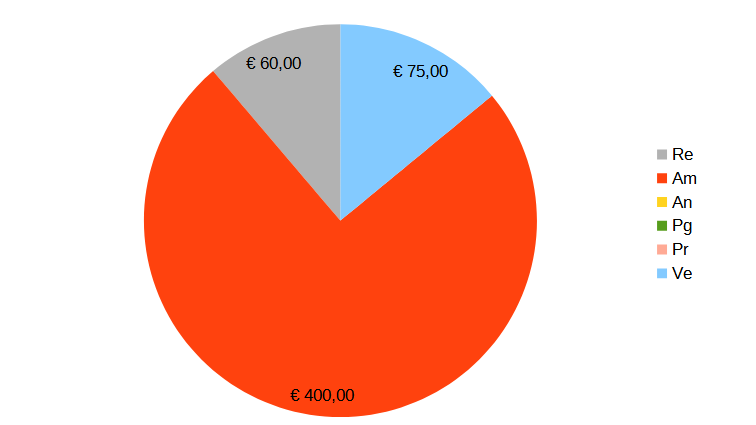
\includegraphics[width=0.8\textwidth]{res/img/grafici/consuntivo-torta-incremento5.png}
	\caption{Preventivo - Incremento V  - costo per ruolo} 
\end{figure}

\newpage
\subsection{Incremento VI}
\subsubsection{Prospetto orario}

\begin{table} [h!]
	\rowcolors{2}{gray!25}{gray!6}
	\begin{center}
		\begin{tabular} { m{3.5cm} c c c c c c c }
			\rowcolor{lightgray}
			\textbf{Nome} & \textbf{Re} & \textbf{Am} & \textbf{An} & \textbf{Pg} & \textbf{Pr} & \textbf{Ve} & \textbf{Totale} \\
			Matteo Alba & 2(+2) & 3(+1) & 0 & 3(+3) & 4(+4) & 8(+8) & 20(+18) \\
		Giacomo Bulbarelli & 0 & 3 & 0 & 3 & 8(-1) & 6 & 20(-1) \\
		Alessandro Chimetto & 0 & 3 & 0 & 2 & 7(-1) & 8 & 20(-1) \\
		Alessandro Dindinelli & 1 & 3 & 0 & 3 & 7 & 6(-1) & 20(-1) \\
		Lucia Fenu & 2 & 4 & 0 & 2 & 4(-1) & 8(+1) & 20 \\
		Paolo Scanferlato & 1 & 3 & 0 & 3 & 5 & 8 & 20 \\
		Valton Tahiraj & 1 & 2 & 0 & 1 & 8(-1) & 8 & 20(-1) \\
		\textbf{Ore totali Ruolo} & \textbf{7(+2)} & \textbf{21(+1)} & \textbf{0} & \textbf{17(+3)} & \textbf{43}& \textbf{52(+8)} & \textbf{140(+14)}
		\end{tabular}
		\caption{Preventivo - Incremento VI - ore per persona/ruolo}
	\end{center}
\end{table}
\begin{figure} [h!]
	\centering
	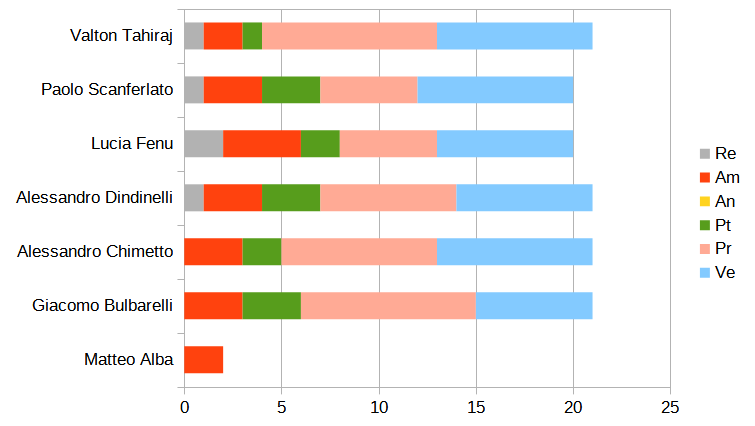
\includegraphics[width=0.8\textwidth]{res/img/grafici/consuntivo-barre- incremento6.png}
	\caption{Preventivo - Incremento VI - ore per persona/ruolo} 
\end{figure}

\newpage
\subsubsection{Prospetto economico}
\begin{table} [h!] % QUESTA RICHIEDE \usepackage{eurosym} IN config.tex
	\rowcolors{2}{gray!25}{gray!6}
	\begin{center}
		\begin{tabular} { m{3cm} >{\centering}m{1.5cm} c }
			\rowcolor{lightgray}
			\textbf{Ruolo} & \textbf{Ore} & \textbf{Costo in \euro} \\
			Responsabile & 7(+2) & 210,00(+60,00) \\
		Amministratore & 21(+1) & 420,00(+20,00)\\
		Analista & 0 & 0,00 \\
		Progettista & 17(+3) & 374,00(+66,00) \\
		Programmatore & 43 & 645,00 \\
		Verificatore & 52(+8) & 780,00(+120,00) \\
		\textbf{Totale} & \textbf{140(+14)} & \textbf{2429,00(+266,00)} \\
		\end{tabular}
		\caption{Preventivo - Incremento VI  - costo per ruolo}
	\end{center}
\end{table}

\begin{figure} [h!]
	\centering
	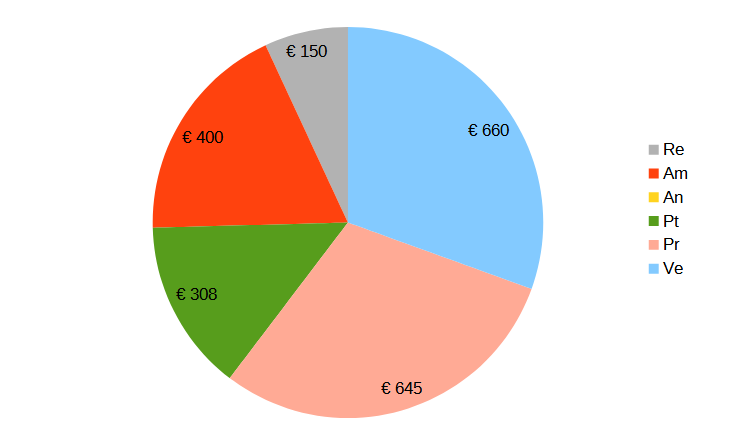
\includegraphics[width=0.8\textwidth]{res/img/grafici/consuntivo-torta-incremento6.png}
	\caption{Preventivo - Incremento VI  - costo per ruolo} 
\end{figure}

\newpage

\subsection{Incremento VII}

\subsubsection{Prospetto orario}

\begin{table} [h!]
	\rowcolors{2}{gray!25}{gray!6}
	\begin{center}
		\begin{tabular} { m{3.5cm} c c c c c c c }
			\rowcolor{lightgray}
			\textbf{Nome} & \textbf{Re} & \textbf{Am} & \textbf{An} & \textbf{Pg} & \textbf{Pr} & \textbf{Ve} & \textbf{Totale} \\
			Matteo Alba & 0 & 5(+5) & 0 & 0 & 2(+2) & 3(+3) & 10(+10) \\
			Giacomo Bulbarelli & 2(+1) & 0(-3) & 0 & 0 & 3(-1) & 5 & 10(-3) \\
			Alessandro Chimetto & 0 & 3(-1) & 0 & 0& 3(-3) & 4(+1) & 10(-3) \\
			Alessandro Dindinelli & 0 & 2 & 0 & 0 & 3(-3) & 5 & 10(-3) \\
			Lucia Fenu & 0 & 3(-2)& 0 & 0 & 3(+1) & 4(-2) & 10(-3) \\
			Paolo Scanferlato & 0(-1) & 2(-2) & 0 &0 & 3(+1) & 5(-1) & 10(-3) \\
			Valton Tahiraj & 2 & 1(-1) & 0 & 0 & 3(-2) & 4 & 10(-3) \\
			\textbf{Ore totali Ruolo} & \textbf{4} & \textbf{16(-4)} & \textbf{0} & \textbf{0} & \textbf{20(-5)}& \textbf{30(+1)} & \textbf{70(-8)}
		\end{tabular}
		\caption{Consentivo - Incremento VII - ore per persona/ruolo}
	\end{center}
\end{table}

\begin{figure} [h!]
	\centering
	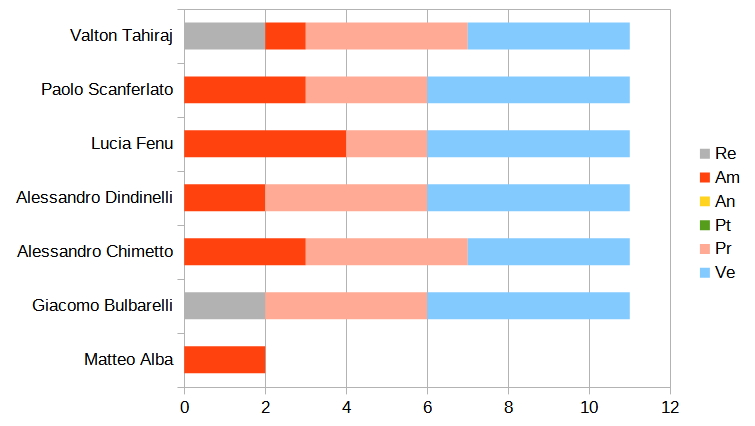
\includegraphics[width=0.8\textwidth]{res/img/grafici/consuntivo-barre-val.png}
	\caption{Consuntivo - Incremento VII - ore per persona/ruolo} 
\end{figure}

\newpage

\subsubsection{Prospetto economico}

\begin{table} [h!] % QUESTA RICHIEDE \usepackage{eurosym} IN config.tex
	\rowcolors{2}{gray!25}{gray!6}
	\begin{center}
		\begin{tabular} { m{3cm} >{\centering}m{1.5cm} c }
			\rowcolor{lightgray}
			\textbf{Ruolo} & \textbf{Ore} & \textbf{Costo in \euro} \\
			Responsabile & 4 & 120,00 \\
			Amministratore & 16(-4) & 320,00(-80,00) \\
			Analista & 0 & 0 \\
			Progettista & 0 & 0 \\
			Programmatore & 20(-5) & 300,00(-75,00) \\
			Verificatore & 30(+1) & 450,00(+15,00) \\
			\textbf{Totale} & \textbf{70} & \textbf{1190,00} \\
		\end{tabular}
		\caption{Consuntivo - Incremento VII - costo per ruolo}
	\end{center}
\end{table}

\begin{figure} [h!]
	\centering
	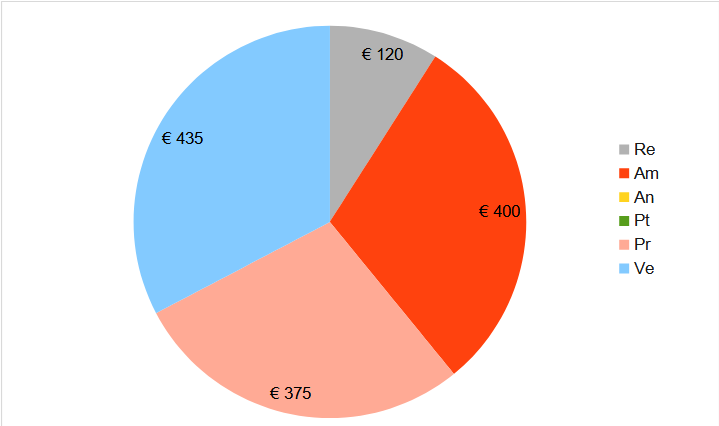
\includegraphics[width=0.8\textwidth]{res/img/grafici/consuntivo-torta-val.png}
	\caption{Consuntivo - Incremento VII - costo per ruolo} 
\end{figure}



\subsubsection{Conclusioni finali incrementi}

Ogni sottogruppo che ha lavorato durante gli Incrementi ha riscontrato alcune difficoltà, aumentando così le ore nel ruolo di Programmatore.
Il riscontro dei rischi non è stato adeguato e dunque ha portato alla creazione di una pianificazione, e di conseguenza un preventivo non al pari dei singoli consuntivi di Incremento.\\
Nonostante ciò, il gruppo ha lavorato bene con continui feedback da e verso i sottogruppi.
\\
Durante gli incrementi finali prima della consegna finale, il gruppo era consapevole del lavoro da portare a termine e dunque la pianificazione è stata rispettata adeguatamente, nonostante la non partecipazione da parte di un componente.\\

 



\newpage

\subsection{Riepilogo}

\subsubsection{Prospetto orario totale di investimento}

\begin{table} [h!]
	\rowcolors{2}{gray!25}{gray!6}
	\begin{center}
		\begin{tabular} { m{3.5cm} c c c c c c c }
			\rowcolor{lightgray}
			\textbf{Nome} & \textbf{Re} & \textbf{Am} & \textbf{An} & \textbf{Pg} & \textbf{Pr} & \textbf{Ve} & \textbf{Totale} \\
			Matteo Alba & 13(+7)& 24(-3)& 17(+4) & 19(+6) & 24(+9) & 43(+12) & 140(+35) \\
			Giacomo Bulbarelli & 14(+5) & 15(-4) & 18 & 29(-10) & 30(-19) & 34(-5) & 140(-33) \\
			Alessandro Chimetto & 9(-1) & 15(-4) & 18(+5) & 25(-14) & 31(-21) & 42(+2) & 140(-33) \\
			Alessandro Dindinelli & 6 & 17(-4) & 16(+2) & 27(-11) & 34(-17)& 40(-3) & 140(-33) \\
			Lucia Fenu & 7(-5) & 19(-11) & 15(+7) & 27(-10) & 29(-10) & 43(-3) & 140(-32) \\
			Paolo Scanferlato & 10 & 20(-7) & 11(+2) & 26(-11) & 27(-12) & 46(-4) & 140(-32) \\
			Valton Tahiraj & 9(+3)& 13(-4) & 14(+4) & 24(-13) & 33(-15) & 47(-8) & 140 \\
			\textbf{Ore totali Ruolo} & \textbf{68(+9)} & \textbf{123(-37)} & \textbf{109(+24)} & \textbf{177(-63)} & \textbf{208(-85)}& \textbf{295(-9)} & \textbf{980(-161)}
		\end{tabular}
		\caption{Consuntivo - Ore totali per persona/ruolo}
	\end{center}
\end{table}

\begin{figure} [h!]
	\centering
	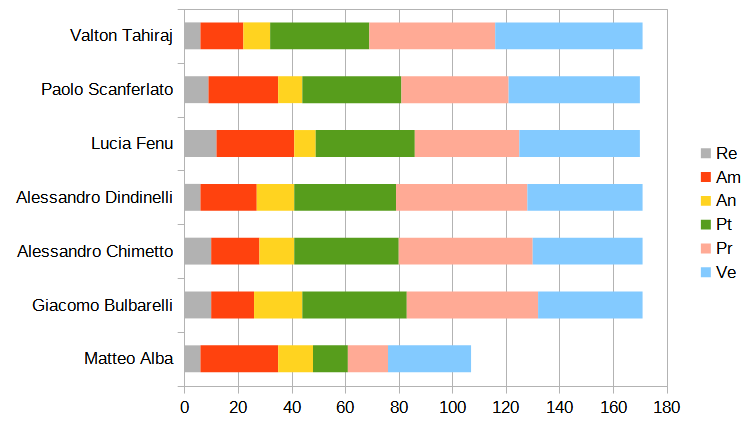
\includegraphics[width=0.8\textwidth]{res/img/grafici/consuntivo-barre-finale.png}
	\caption{Consuntivo - Ore totali per persona/ruolo} 
\end{figure}

\newpage

\subsubsection{Prospetto economico totale di investimento}

\begin{table} [h!] % QUESTA RICHIEDE \usepackage{eurosym} IN config.tex
	\rowcolors{2}{gray!25}{gray!6}
	\begin{center}
		\begin{tabular} { m{3cm} >{\centering}m{3cm} c }
			\rowcolor{lightgray}
			\textbf{Ruolo} & \textbf{Ore} & \textbf{Costo in \euro} \\
			Responsabile & 68(+9) & 2040,00(+270,00) \\
			Amministratore & 123(-37) & 2380,00(-820,00) \\
			Analista & 109(+24) & 2725,00(+600,00) \\
			Progettista & 177(-63) & 3872,00(-1408,00) \\
			Programmatore & 208(-85) & 3075,00(-1320,00) \\
			Verificatore & 295(-9) & 4365,00(-195,00) \\
			\textbf{Totale} & \textbf{980(-161)} & \textbf{18457,00(-2873,00)} \\
		\end{tabular}
		\caption{Consuntivo - Costo totale per ruolo}
	\end{center}
\end{table}

\begin{figure} [h!]
	\centering
	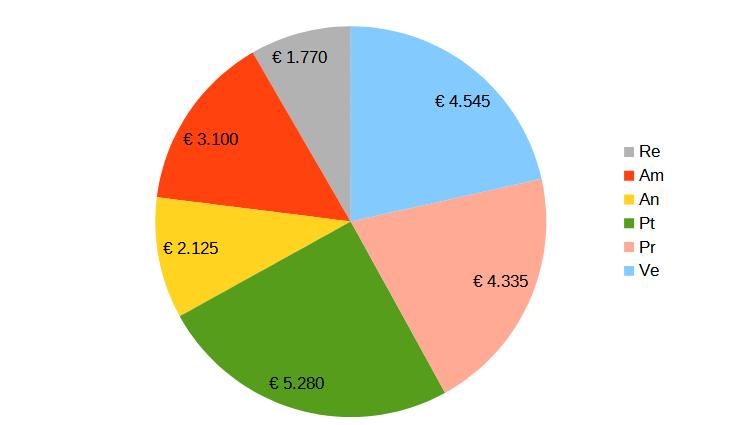
\includegraphics[width=0.8\textwidth]{res/img/grafici/consuntivo-torta-costo finale.png}
	\caption{Consuntivo - Costo totale per ruolo} 
\end{figure}

\newpage

\subsubsection{Prospetto orario rendicontato}

\begin{table} [h!]
	\rowcolors{2}{gray!25}{gray!6}
	\begin{center}
		\begin{tabular} { m{3.5cm} c c c c c c c }
			\rowcolor{lightgray}
			\textbf{Nome} & \textbf{Re} & \textbf{Am} & \textbf{An} & \textbf{Pg} & \textbf{Pr} & \textbf{Ve} & \textbf{Totale} \\
			Matteo Alba & 11(+5) & 16(+4) & 9& 19(+6) & 24(+9) & 29(+11) & 108(+35) \\
			Giacomo Bulbarelli &7(+1) & 7(-3) & 6(+2) & 29(-10) & 30(-19) & 29(-4) & 108(-33) \\
			Alessandro Chimetto &2 & 10(-2) & 6(+2) & 25(-14) & 31(-21) & 34(+2) & 108(-33) \\
			Alessandro Dindinelli & 3& 13(-1) & 3 & 27(-11) & 34(-17) & 28(-4) & 108(-33) \\
			Lucia Fenu & 6(-2) & 13(-5) & 2(-1) & 27(-10) & 29(-10) & 31(-4) & 108(-32)\\
			Paolo Scanferlato & 5(-1) & 13(-3) & 3 & 26(-11) & 27(-12) & 34(-5) & 108(-32) \\
			Valton Tahiraj & 3 & 8(-2) & 4(+2) & 24(-13) & 33(-15) & 36(-5) & 108(-33) \\
			\textbf{Ore totali Ruolo} & \textbf{37(+3)} & \textbf{80(-12)} & \textbf{33(+5)} & \textbf{177(-63)} & \textbf{208(-85)}& \textbf{221(-9)} & \textbf{756(-161)}
		\end{tabular}
		\caption{Consuntivo - Ore totali rendicontate per persona/ruolo}
	\end{center}
\end{table}

\begin{figure} [h!]
	\centering
	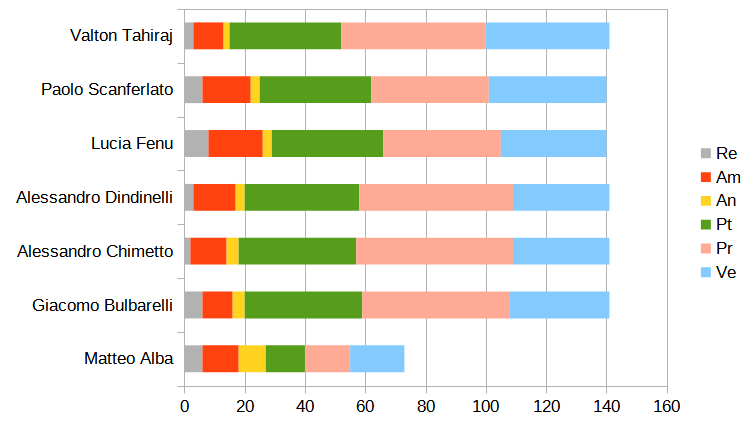
\includegraphics[width=0.8\textwidth]{res/img/grafici/consuntivo-barre-finale-rendicontato.png}
	\caption{Consuntivo - Ore totali rendicontate per persona/ruolo} 
\end{figure}

\newpage

\subsubsection{Prospetto economico rendicontato}

\begin{table} [h!] % QUESTA RICHIEDE \usepackage{eurosym} IN config.tex
	\rowcolors{2}{gray!25}{gray!6}
	\begin{center}
		\begin{tabular} { m{3cm} >{\centering}m{1.5cm} c }
			\rowcolor{lightgray}
			\textbf{Ruolo} & \textbf{Ore} & \textbf{Costo in \euro} \\
			Responsabile & 37(+3) & 1110,00(+90,00) \\
			Amministratore & 80(-12) & 1600,00(-240,00) \\
			Analista & 33(+5) & 825,00(+125,00) \\
			Progettista & 177(-63) &3894,00(1386,00) \\
			Programmatore & 208(-85) & 3120,00(-1275,00) \\
			Verificatore & 221(-9) & 3315,00(-135,00) \\
			\textbf{Totale} & \textbf{707} & \textbf{13864,00(-2821,00)} \\
		\end{tabular}
		\caption{Consuntivo - Prospetto economico rendicontato per ruolo}
	\end{center}
\end{table}

\begin{figure} [h!]
	\centering
	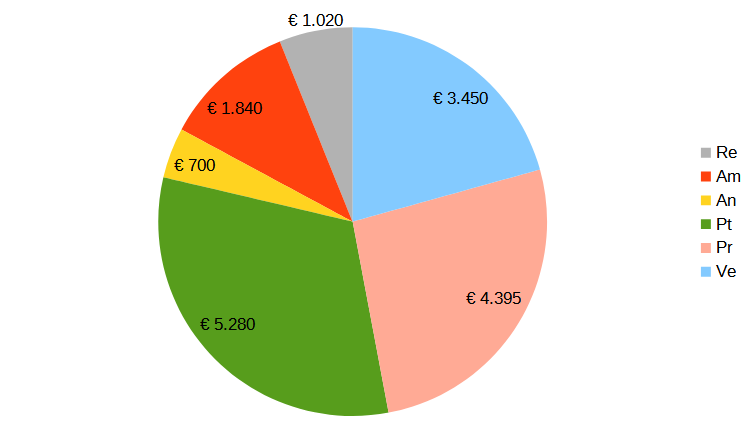
\includegraphics[width=0.8\textwidth]{res/img/grafici/consuntivo-torta-costo finale-rendicontato.png}
	\caption{Consuntivo - Prospetto economico rendicontato per ruolo} 
\end{figure}

\clearpage
\subsection{Preventivo a finire}
Di seguito il preventivo a finire sulla base dei consuntivi fino ad ora svolti.
\begin{table} [h!]
	\begin{center}
		\rowcolors{2}{gray!25}{gray!6}
		\begin{tabular} { m{8 cm} c c c  }
			\rowcolor{lightgray}
			\textbf{Periodo}  & \textbf{Preventivo in \euro} & \textbf{Consuntivo in \euro} \\
			Analisi dei Requisiti   			& 3905,00     & 3775,00 \\
			Analisi di dettaglio  				& 895,00     & 870,00 \\
			Codifica Technology Baseline        & 3633,00     & 3590,00 \\
			Progettazione Architetturale		&3017,00		&  4536,00\\
			Totale Incrementi					& 7217,00		&	8559,00\\
			\textbf{Totale}     & \textbf{18457,00}         & \textbf{21330,00}   \\
			\textbf{Rendicontato}  & \textbf{13864,00}          & \textbf{16685,00}   \\
			
			
		\end{tabular}
		\caption{Preventivo a finire }
	\end{center}
\end{table}

\subsection{Costo finale}
Il costo finale del prodotto, rimane quanto pattuito con il proponente: 13124,00 \euro.